% This file was created with tikzplotlib v0.10.1.
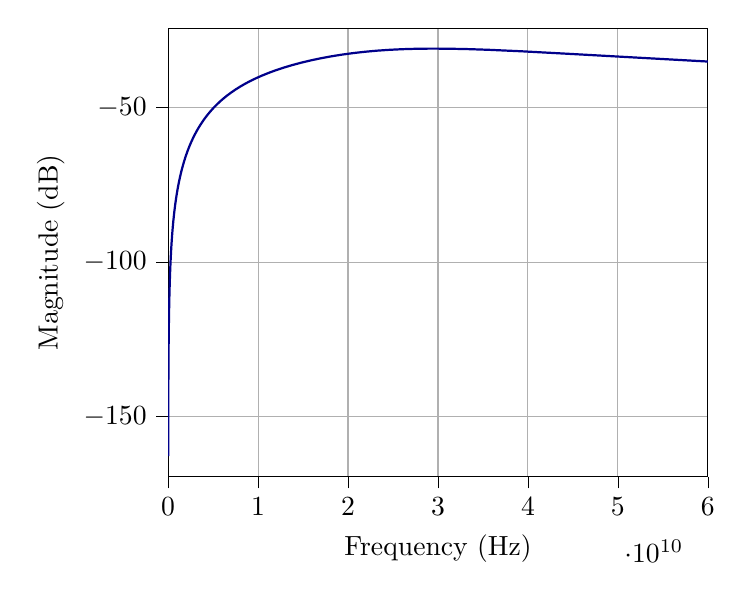
\begin{tikzpicture}

\definecolor{darkblue}{RGB}{0,0,139}
\definecolor{darkgray176}{RGB}{176,176,176}

\begin{axis}[
tick align=outside,
tick pos=left,
x grid style={darkgray176},
xlabel={Frequency (Hz)},
xmajorgrids,
xmin=10000000, xmax=60000000000,
xtick style={color=black},
xtick={0,10000000000,20000000000,30000000000,40000000000,50000000000,60000000000},
%xticklabels={0,10,20,30,40,50,60},
y grid style={darkgray176},
ylabel={Magnitude (dB)},
ymajorgrids,
ymin=-169.394705, ymax=-24.289195,
ytick style={color=black}
]
\addplot [thick, darkblue]
table {%
10000000 -162.79899597168
20000000 -147.266998291016
30000000 -139.182006835938
40000000 -133.764007568359
50000000 -129.680999755859
60000000 -126.397003173828
70000000 -123.649002075195
80000000 -121.281997680664
90000000 -119.204002380371
100000000 -117.350997924805
110000000 -115.678001403809
120000000 -114.15299987793
130000000 -112.751998901367
140000000 -111.457000732422
150000000 -110.251998901367
160000000 -109.125999450684
170000000 -108.068000793457
180000000 -107.071998596191
190000000 -106.128997802734
200000000 -105.236000061035
220000000 -103.575996398926
240000000 -102.061996459961
260000000 -100.668998718262
280000000 -99.3798980712891
300000000 -98.1801986694336
320000000 -97.0581970214844
340000000 -96.0045013427734
360000000 -95.0111999511719
390000000 -93.6204986572266
420000000 -92.3331985473633
450000000 -91.1351013183594
480000000 -90.0145034790039
510000000 -88.9620971679688
550000000 -87.6516036987305
590000000 -86.4335021972656
630000000 -85.2957000732422
670000000 -84.2282028198242
720000000 -82.9804992675781
770000000 -81.8170013427734
820000000 -80.7272033691406
880000000 -79.5046005249023
940000000 -78.3630981445312
1010000000 -77.1209030151367
1080000000 -75.9627990722656
1160000000 -74.7287979125977
1240000000 -73.5781021118164
1330000000 -72.3703994750977
1420000000 -71.2431030273438
1520000000 -70.072998046875
1630000000 -68.8733978271484
1740000000 -67.7540969848633
1860000000 -66.6130981445312
1990000000 -65.4598007202148
2130000000 -64.302001953125
2280000000 -63.1463012695312
2440000000 -61.9981994628906
2609999872 -60.8620986938477
2790000128 -59.74169921875
2980000000 -58.6398010253906
3180000000 -57.5587005615234
3400000000 -56.4515991210938
3630000128 -55.375
3880000000 -54.2872009277344
4140000000 -53.2359008789062
4419999744 -52.1842002868652
4729999872 -51.1052017211914
5059999744 -50.0432014465332
5400000000 -49.0307998657227
5769999872 -48.0119018554688
6169999872 -46.9954986572266
6600000000 -45.989200592041
7049999872 -45.0196990966797
7550000128 -44.0299987792969
8040000000 -43.1380996704102
8579999744 -42.2332000732422
9189999616 -41.2969017028809
9799999488 -40.4398994445801
10449999872 -39.6025009155273
11189999616 -38.7322998046875
11969999872 -37.8983001708984
12880000000 -37.0190010070801
13829999616 -36.1945991516113
14800000000 -35.4392013549805
15900000256 -34.6759986877441
16990000128 -34.0075988769531
18190000128 -33.3633995056152
19330000896 -32.8334007263184
20559998976 -32.3446006774902
21870000128 -31.9127006530762
23289999360 -31.540599822998
24600000512 -31.2791004180908
26030000128 -31.0757007598877
27640000512 -30.9386005401611
29159999488 -30.8871994018555
30960001024 -30.9095001220703
33209999360 -31.0396003723145
35579998208 -31.269100189209
39310000128 -31.7567005157471
45070000128 -32.6605987548828
60000002048 -35.0740013122559
};
\end{axis}

\end{tikzpicture}
